\chapter{Verification and Case Studies} \label{chapter:case-studies}

\section{Introduction}
We present a series of numerical simulations to verify and validate our model in this chapter. Plume-SPH has been verified by comprehensive 1D shock tube tests in Chapter \ref{chapter:GSPH-RSPH}. In this chapter, Plume-SPH will be further verified by a JPUE simulation. Velocity and mass fraction distribution both along the central axis and cross transverse are compared with experimental results. The pattern of ambient particles entrainment is also clearly shown. Then a simulation of representative strong volcanic plume, the Pinatubo eruption at June 15th 1991, is conducted. Integrated local variable are comparable with simulation results from existing 3D plume models.
The output of Pinatubo simulation will also be used in Chapter \ref{chapter:ash-transportation} to create initial condition for ash transportation simulation of Pinatubo eruption.

\section{Simulation of JPUE}
JPUE can be considered as a simplified volcanic plume. While the effect of stratified atmosphere and the effect of expansion due to high temperature in volcanic plume are not represented, JPUE reproduces the entrainment due to turbulent mixing which is one of the key elements in volcanic plume development. There exist consistently good experimental data \citep { list1982turbulent,dimotakis1983structure, papanicolaou1988investigations, ezzamel2015dynamical} that describe the JPUE flow field giving an insight into details of JPUE, such as transverse velocity and concentration profile. In this section, we verify that our code and the $SPH-\varepsilon$ turbulence model is able to reproduce feature of turbulent entrainment by a JPUE simulation.

As many of these experiments were conducted with liquid, we replace the original equation of state (Eq. (\ref{eq:EOS})) with a weakly compressible Tait equation of state \citep {becker2007weakly} (see Eq. (\ref{eq:EOS-Tait})) to avoid solving the Poisson equation.
\begin{equation}
p=B\left[\left(\dfrac{\rho}{\rho_0}\right)^{\gamma}-1\right]
\label{eq:EOS-Tait}
\end{equation}
with $\gamma=7$ and $B$ is evaluated by:
\begin{equation}
B=\dfrac{\rho_0 c^2}{\gamma}
\end{equation}
where $c$ is the speed of sound in the liquid. The energy equation is actually decoupled from the momentum conservation equation and the mass conservation equation by using this ESO. In addition, the "atmosphere" is assumed to be uniform and gravity is set to be zero. We set the temperature and density of ejected material the same as surrounding ambient. This further simplifies the scenario for the convenience of studying turbulent mixing. 

One overall feature of JPUE is "self-similarity" which means that the evolution of the JPUE is determined solely by the local scale of length and velocity which theoretically accounts for the fact that the rate of entrainment at the edge of JPUE is proportional to a characteristic velocity at each height. As a result, physical and numerical experiments do not necessarily to have exactly the same setups and are compared on a non-dimensional basis.

\begin{table}[htp]
\centering
	\begin{centering}
      \caption{Eruption condition for Plume and JPUE simulation}		
	  \begin{tabular}{lrrr}
	    \hline
	    Parameters & Units  & JPUE & Plume \\
	    \hline
	    Vent velocity          & $m\cdot s^{-1}$  & 500               & 275 \\
	    Vent gas mass fraction &                  & 1.0               & 0.05 \\
	    Vent Temperature       & $K$              & 273               & 1053 \\
	    Vent height            & $m$              & 0                 & 1500 \\
	    Mass discharge rate    & $kg\cdot s^{-1}$ & $5.47 \times 10^7$ & $1.5 \times 10^9$\\
	    \hline
	  \end{tabular}
	  \label{tab:input_parameters}
	\end{centering}
\end{table}

\begin{figure}
    \centering
    \begin{minipage}{.49\textwidth}
        \centering
        \includegraphics[width=0.99 \textwidth]{Chapter-6/Figures/vel_cross}
    \end{minipage}%
    \begin{minipage}{.49 \textwidth}
        \centering
        \includegraphics[width=0.99 \textwidth]{Chapter-6/Figures/conc_cross}
    \end{minipage}%  
    \caption{Dimensionless concentration and velocity distribution across the cross-section.}
    \label{fig:JPUE_cross-section}
\end{figure}

\begin{figure}
    \centering
    \begin{minipage}{.49\textwidth}
        \centering
        \includegraphics[width=0.99 \textwidth]{Chapter-6/Figures/velo_along_axis}
    \end{minipage}%
    \begin{minipage}{.49 \textwidth}
        \centering
        \includegraphics[width=0.99 \textwidth]{Chapter-6/Figures/conc_along_axis}
    \end{minipage}%  
    \caption{The left plot is normalized jet width (which determined based on velocity) along the centerline. The right plot shows normalized concentration along the centerline.}
    \label{fig:JPUE_along-axis}
\end{figure}

A three dimensional axisymmetric JPUE which ejects from a round vent is simulated with eruption parameters listed in Table \ref{tab:input_parameters}. Material properties of water are used as material properties for both phases. The results are compared with experiments \citep {george1977turbulence, papanicolaou1988investigations} for verification purposes. Experimental data of concentration and velocity distribution across the cross-section were fit into a Gaussian profile (See Eq. (\ref{eq:JPUE-experiment-fit-corss})) by \citet{papanicolaou1988investigations} and  \citet{ george1977turbulence} even though the actual profile are slightly different from the Gaussian profile.

\begin{equation}
\dfrac{\varphi}{\varphi_c}=exp \left[-coef\left( \left(\dfrac{r}{z}\right)^2\right)\right]
\label{eq:JPUE-experiment-fit-corss}
\end{equation}

where $\varphi$ is either velocity or concentration, the subscript $c$ represents the centreline. $r$ is the distance from the centreline on any cross-section. $z$ is the axial distance from the origin of the jet transverse section under consideration. 
The coefficient $coef$ for concentration is 80 and 50 respectively according to \citet{george1977turbulence} and \citet{papanicolaou1988investigations}.
$coef$ for velocity is 90 and 55 respectively according to \citet{george1977turbulence} and \citet{papanicolaou1988investigations}. 

\citet{papanicolaou1988investigations} also fit concentration distribution and jet width based on velocity along centerline into a straight line (See Eq. (\ref{eq:JPUE-experiment-fit-along-axis})).. 

\begin{equation}
\dfrac{\varphi_0}{\varphi_c}=slope \left(\dfrac{z}{D} + intercept \right)
\label{eq:JPUE-experiment-fit-along-axis}
\end{equation}

where subscript $0$ represents the cross-sectionally averaged exit value, $D$ is the diameter of vent. 
$slope$ for jet width based on velocity is 0.104 and for concentration is 0.157. 
$intercept$ for jet width based on velocity is 2.58 while that for the concentration is 4.35.

Although both velocity and concentration are found to be well matched with experimental results, a small disparity in both velocity and concentration are observed near the boundary of the jet. Which is possibly caused by overestimating of the drag effect by standard SPH \citep {ritchie2001multiphase}. \citet {ritchie2001multiphase} also proposed an alternative way for density update which relieved the overestimating of the drag effect. However, how well does his method conserve mass is not clear. There are several other factors that might also attribute to such disparity. Reynolds number is not reported in many experiments assuming a high enough Reynolds number. In addition, some details of the experiments, such as exit velocity profile and viscosity of the experimental liquid, are not reported. These factors prevent us from numerically reproducing these experiments in an exact way as they were conducted. However, the features of JPUE are correctly reproduced with our code.

We also investigated the mixing due to turbulence in JPUE simulation by checking the mixture of the two phases. It is shown in Fig. \ref{fig:Turb_mixing} that the ejected material and ambient fluids are mixed through eddies at the outer shear region. And the inner dense core dispersed gradually due to erosion of the outer shear region. Hence, our confidence in the numerical correctness of our code is greatly reinforced.

\begin{figure}
\centering
\includegraphics[width=0.65 \textwidth]{Chapter-6/Figures/JPUE_entrainment.png}
\caption{The left figure shows particle distribution. Particles of phase 1 (blue) are gradually entrained and mixed with erupted particles (red) as jet flows down stream. The right figure shows the mass fraction of erupted material at the moment corresponding to the left figure.}
\label{fig:Turb_mixing}
\end{figure}

\section{Pinatubo eruption in June 15 1991}
The development of a volcanic plume is more complicated than JPUE in several aspects. Besides turbulent entrainment of ambient fluids, development of volcanic plume also involves heating up of entrained air and expanding in a stratified atmosphere. A strong eruption (climactic phase of Mountain Pinatubo eruption in Jun 15th 1991), during which the effect of wind field is relatively neglectable, is tested in this section for the purpose of further verification and validation.
Both global variable and local variables are compared with existing models.

\subsection{Input parameters}
\label{input-parameter}
Eruption parameters, material properties and atmosphere are chosen to be the same as the strong plume no wind case in a comparison study on eruptive column models by \citet {costa2016results}. Eruption conditions are listed in Table \ref{tab:input_parameters}. As our model does not distinguish solid particles of different sizes, only mass fraction of solids of all size is used in simulation even though two size classes were provided by \citet {costa2016results}. The density of erupted material at the vent and radius of the vent can be computed from the given parameters. The eruption pressure is assumed to be as the same as pressure of ambient at the vent and hence is not given in the table. The vertical profiles of atmospheric properties were obtained based on the reanalysis data from ECMWF (European Centre for Medium-Range Weather Forecasts) for the period corresponding to the climactic phase of the Pinatubo eruption (Philippines, 15 June 1991). These conditions are more typical of a tropical atmosphere (see Fig. 1B in \citep{costa2016results}).  
Vertical distribution of temperature, pressure and density is used to establish stratified atmosphere. Wind velocity and specific humidity are not used in our simulation even though they were also provided in Fig. 1B \citep{costa2016results}. Material properties, shown in Table \ref{tab:material_properties}, are selected based on properties of Pinatubo and Shinmoe-dake eruption. Other material properties not given in the table can be inferred from these given parameters.

\begin{table}[htp]
\centering
	\begin{centering}
      \caption{Material properties for Plume and JPUE simulation}		
	  \begin{tabular}{lrrr}
	    \hline
	    Parameters & Units  & Value \\
	    \hline
	    	Specific heat of gas at constant volume     & $J \cdot kg^{-1}\cdot K^{-1}$& 717     \\
	    Specific heat of air at constant volume     & $J \cdot kg^{-1}\cdot K^{-1}$& 1340    \\
	    	Specific heat of solid                      & $J \cdot kg^{-1}\cdot K^{-1}$& 1100    \\
	    	Specific heat of gas at constant pressure   & $J \cdot kg^{-1}\cdot K^{-1}$& 1000    \\
	    	Specific heat of air at constant pressure   & $J \cdot kg^{-1}\cdot K^{-1}$& 1810    \\
	    	Density of air at vent height               & $kg \cdot m^{-3}$       & 1.104   \\
	    Pressure at vent height                        & $Pa$              & 84363.4 \\
	    \hline
	  \end{tabular}
	  \label{tab:material_properties}
	\end{centering}
\end{table}

Fig. \ref{fig:pinatubo-simulation-results-vis} shows the mass fraction of simulated volcanic plume at 300s after eruption, at which time the plume starts spreading radially. A contour plot of the mass fraction on the vertical cross-section (y-z plane) is also provided. The zoomed view of the quivier plot shows detailed entrainment of air at the margin of the plume.

\begin{figure}
    \centering
    \begin{minipage}{.45\textwidth}
        \centering
        \includegraphics[width=0.99 \textwidth]{Chapter-6/Figures/mssfrc-Diverging}
    \end{minipage}%
    \begin{minipage}{.45 \textwidth}
        \centering
        \includegraphics[width=0.99 \textwidth]{Chapter-6/Figures/mssfrc-Diverging-cut}
    \end{minipage}%
    \\
    \begin{minipage}{.45 \textwidth}
        \centering
        \includegraphics[width=0.99 \textwidth]{Chapter-6/Figures/gmd-mssfrc-xz}
    \end{minipage}% 
    \begin{minipage}{.45 \textwidth}
        \centering
        \includegraphics[width=0.99 \textwidth]{Chapter-6/Figures/gmd-mssfrc-xz-zoomed}
    \end{minipage}%  
    \caption{Mass fraction for $t=300s$ after eruption. Figures on the first row are visualization of SPH simulation results. The figure on the up right corner is visualization of a slice of the computational. The lowest portion of the plume represents erupted material in eruption vent (the underground portition). Figures at the second row show contour of mass fraction and velocity quiver on x-z plane. These figures are plotted utilizing post-processed data (see Appendix \ref{app:project-SPH-grid}). The contour levels in the plots are $0.00001, 0.0001, 0.001, 0.1, 0.3, 0.75, 0.95$. The figure on the lower right corner is a zoomed view of velocity quivier showing plume expansion and entrainment of air.}
    \label{fig:pinatubo-simulation-results-vis}
\end{figure}

\subsection{Global and local variables}
One of the key global quantities of great interest is the altitude to which the plume rises. The top height predicted by our model is around 40 km which agrees with other plume models. For example, the height predicted by PDAC is 42500 m, by SK-3D is 39920 m, by ATHAM is 33392 m, by AHSEE is 36700 m. As for local variables, the profiles of integrated temperature, density, mass fraction of entrained air, gas mass fraction, mass fraction of solid and the radius of the plume as a function of height are compared with existing 3D models in Fig. \ref{fig:strong_local_temp} $\sim$ \ref{fig:strong_local_radius}. To get rid of significant fluctuations in time and space we conducted a time averaging and spatial integration of the dynamic 3D flow fields following \citet {cerminara2016large}.

As particles distribute irregularly in the space in SPH simulation results. We need to project simulation results (on irregular particles) onto a pre-defined grid before doing time average and spatial integration. See appendix A for more details of post processing.

The profiles of local variables match well with simulation results of existing 3D models in a general sense. The basic phenomena in volcanic plume development are correctly captured by our model.

\begin{figure}
\center
\includegraphics[width=0.5 \textwidth]{Chapter-6/Figures/Temp}
\caption{Temperature as a function of height}
\label{fig:strong_local_temp}
\end{figure}

\begin{figure}
\includegraphics[width=0.99 \textwidth]{Chapter-6/Figures/msfrac}
\caption{The mass fraction of entrained air, gas, and solid as a function of height.}
\label{fig:strong_plume_mass_fraction}
\end{figure}

As the height increases, the amount of entrained air also increases. Around the neutral height, where the umbrella expands, the entrainment of air shows a slight decrease due to lack of air surrounding the column at that height. The profile for gas, which account for both air and vapor, shows a very similar tendency as that of entrained air. Recall that vapor condensation is not considered in our model. In addition, we assume that erupted material behaves like a single-phase fluid. So the mass fraction of gas is simply a function of entrained air (Eq. (\ref{eq:gas-frac-express})).
\begin{equation}
\xi_a + \xi_g = \xi_a + \left(1-\xi_a\right) \xi_{g0}
\label{eq:gas-frac-express}
\end{equation}
 
Among these 3D models, ATHAM takes vapor condensation into account and Eq. (\ref{eq:gas-frac-express}) does not hold for ATHAM. However, the profile of entrained air and profile of gas predicted by ATHAM are still very close to each other which implies that ignoring of water phase change is a valid assumption for eruptions similar to this test case (strong plume with erupted water fraction in erupted material less than 5\%). This observation can be explained by the fact that air occupies a larger portion of the gas and ignoring of phase change of vapor (which is only a small portion of gas) causes slight influence on plume development. As for mass fraction of solid, similarly, Eq. (\ref{eq:solid-frac-express1}) and Eq. (\ref{eq:solid-frac-express2}) hold for our model. 
\begin{equation}
\xi_s = \left(1 - \xi_a\right) \left(1- \xi_{g0}\right)
\label{eq:solid-frac-express1}
\end{equation}
\begin{equation}
\xi_s = 1 - \left(\xi_a + \xi_g\right)
\label{eq:solid-frac-express2}
\end{equation}

PDAC, which treats particles of two different sizes as two separate phases, predicted a similar mass fraction profile. That implies that assumption of dynamic equilibrium in our model is at least valid for eruptions similar to the test case.

With more cool air entrained into the plume and mixing with the hot erupted material, the temperature of the plume decreases as the height increases as shown in Fig. \ref{fig:strong_local_temp}. In the meanwhile, bulk density decrease due to entrainment and expansion (Fig. \ref{fig:strong_local_density}).
\begin{figure}
\center
\includegraphics[width=0.5 \textwidth]{Chapter-6/Figures/density_strong}
\caption{Density of the strong plume without wind after reaching its top height}
\label{fig:strong_local_density}
\end{figure}
\begin{figure}
\center
\includegraphics[width=0.5 \textwidth]{Chapter-6/Figures/radius_strong}
\caption{Radius of the strong plume without wind after reaching its top height.}
\label{fig:strong_local_radius}
\end{figure}
Our model adopts the same assumptions and governing equations as SK-3D. However, there is still a obvious disparity between the profiles of local variables of our model and SK-3D. One of the big differences between these two models is that we adopt a LANS type of turbulence model while SK-3D adopts a LES (large eddy simulation) turbulence model. This implies that choice of turbulence model might play a critical role in plume simulation.

%\subsection{Resolution sensitivity}
%The Pinatubo eruption is simulated with different resolution (smoothing length). The neutral buoyancy level (NBL) of the plume, at which height the plume expands radially, is used as the property of interest in the resolution sensitivity study. Smoothing lengths and obtained NBLs are list in the Table \ref{tab:sml-sensitivity}. Another consideration while picking up smoothing length is to make sure that particle for phase 2 (the erupted material) could symmetrically fill the eruption conduit of given radius. Considering various smoothing lengths can break down the conservation properties of current SPH formulations, large ratio between smoothing length of air particles and smoothing length of erupted material particles is avoided.
%
%\begin{table}[htp]
%\centering
%	\begin{centering}
%      \caption{Sensitivity of NBL with respect to smoothing length}		
%	  \begin{tabular}{lp{2.5cm}p{3.5cm}p{2.2cm} p{2.2cm}}
%	    \hline
%	           & Smoothing \newline length (air) & Smoothing length \newline (Erupted material) & NBL lower & NBL upper\\
%	    \hline
%	    Case 1 & 170 m & 17.5 km & 19.5.0 km &  \\
%	    Case 2 & 300 m & 17.5 km & 19.5 km &  \\
%	    Case 3 & 400 m & 17.0 km & 19.0 km &  \\
%	    Case 4 & 600 m & 15.5 km & 17.5 km &  \\
%	    \hline
%	  \end{tabular}
%	  \label{tab:sml-sensitivity}
%	\end{centering}
%\end{table}
%
%As being showing in the table \ref{tab:sml-sensitivity}, the NBL of plume is loosely associated with resolution. When smoothing length of air is $170 m$, $300 m$ and $400 m$ respectively, the predicted NBLs are all between $17 km$ ~ $25 km$, which consistent measurements based on different techniques \citep[][e.g.]{defoor1992early, deshler1992balloonborne, self1993atmospheric}. However, when attemptting with air particle smoothing length of $600 m$, there is a relatively obvious drop in term of NBL, even though it is still within reasonable range. Possible reason for such changes in forecasted NBL might not be the resolution. When taking $600 m$ as smoothing length of air particles, there are much fewer particles in the eruption conduit leading to a poorly representing of the erupted material. So we can conclude that one constrain for choosing smoothing length is to make sure that there are enough particles in the conduit.

\subsection{Short period eruption}
\begin{figure}
    \centering
    \begin{minipage}{.33\textwidth}
        \centering
        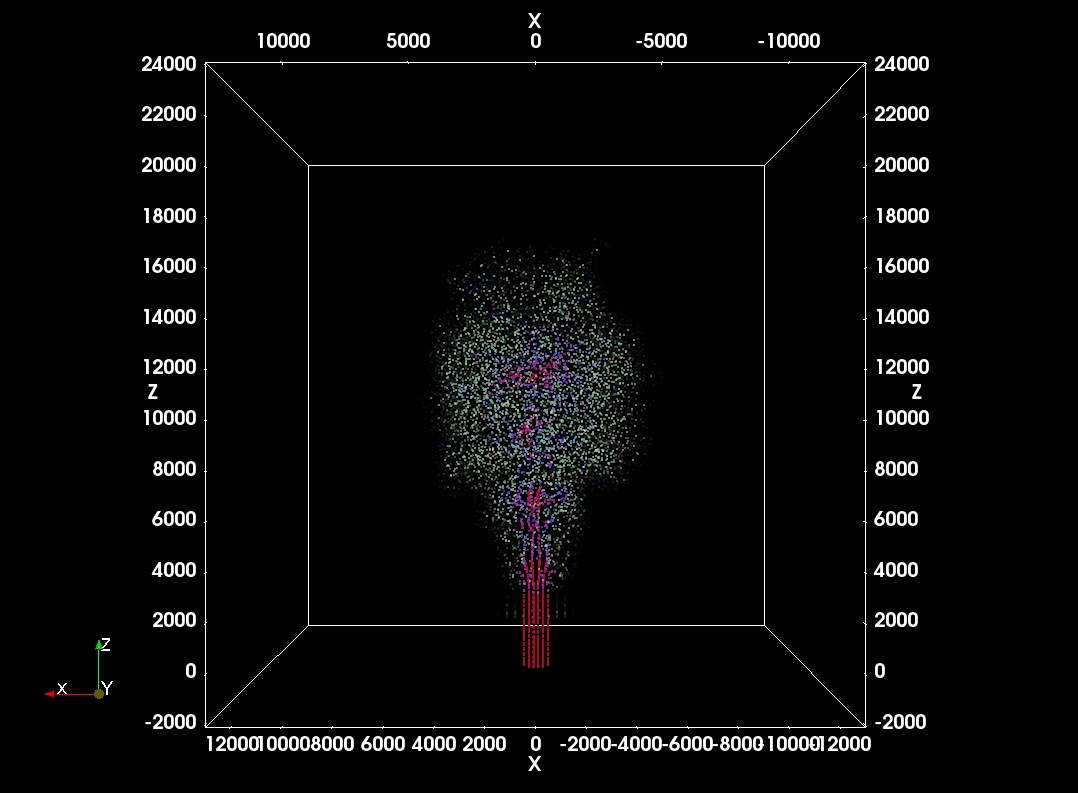
\includegraphics[width=0.99 \textwidth]{Chapter-6/Figures/ShortErupt/Erupt100_t100}
    \end{minipage}%
    \begin{minipage}{.33 \textwidth}
        \centering
        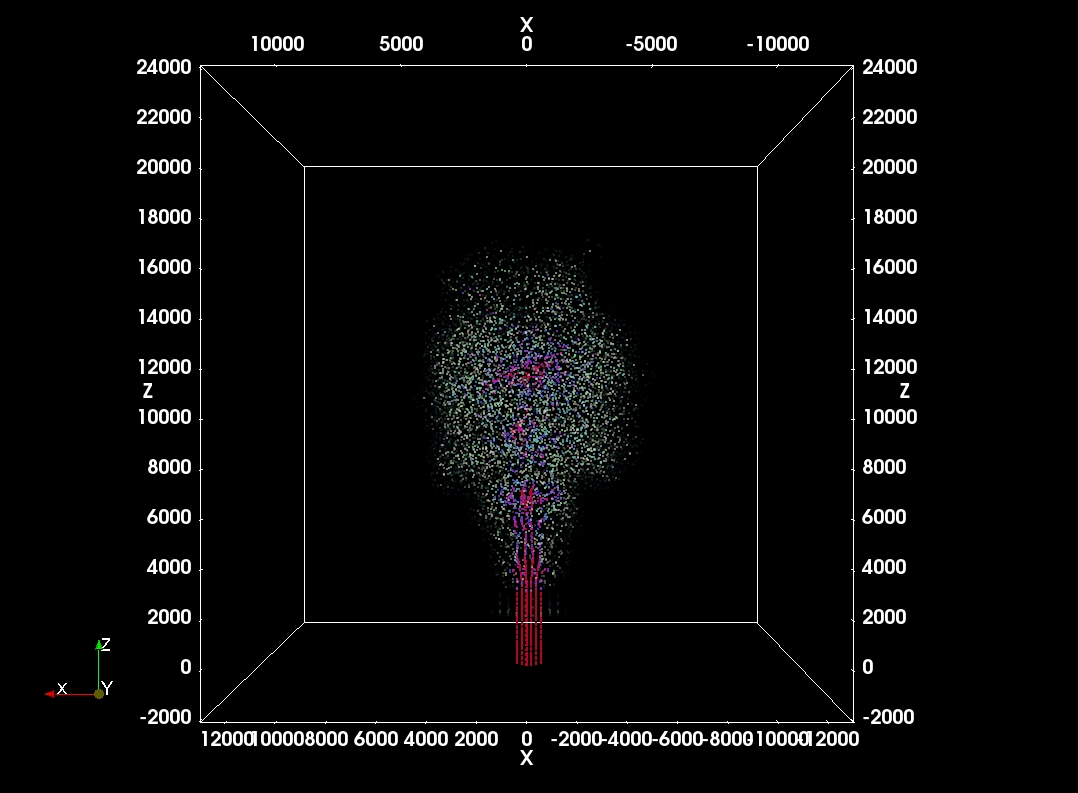
\includegraphics[width=0.99 \textwidth]{Chapter-6/Figures/ShortErupt/Erupt300_t100}
    \end{minipage}%
    \\
    \begin{minipage}{.33\textwidth}
        \centering
        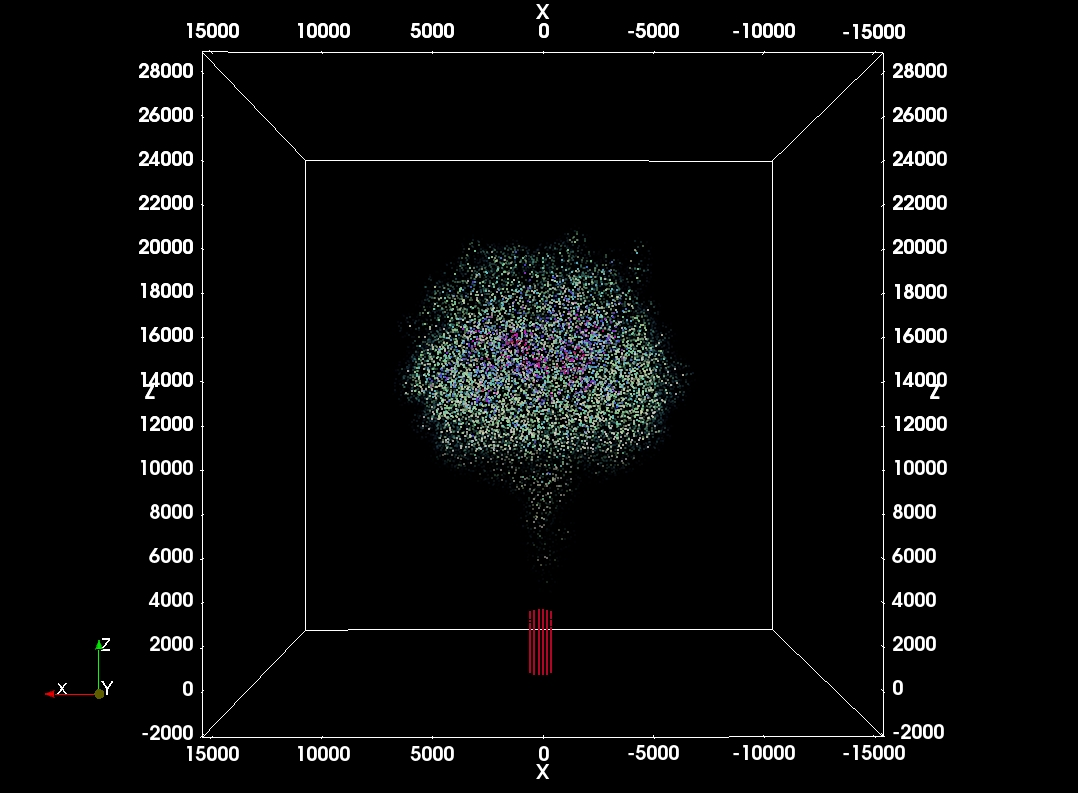
\includegraphics[width=0.99 \textwidth]{Chapter-6/Figures/ShortErupt/Erupt100_t150}
    \end{minipage}%
    \begin{minipage}{.33 \textwidth}
        \centering
        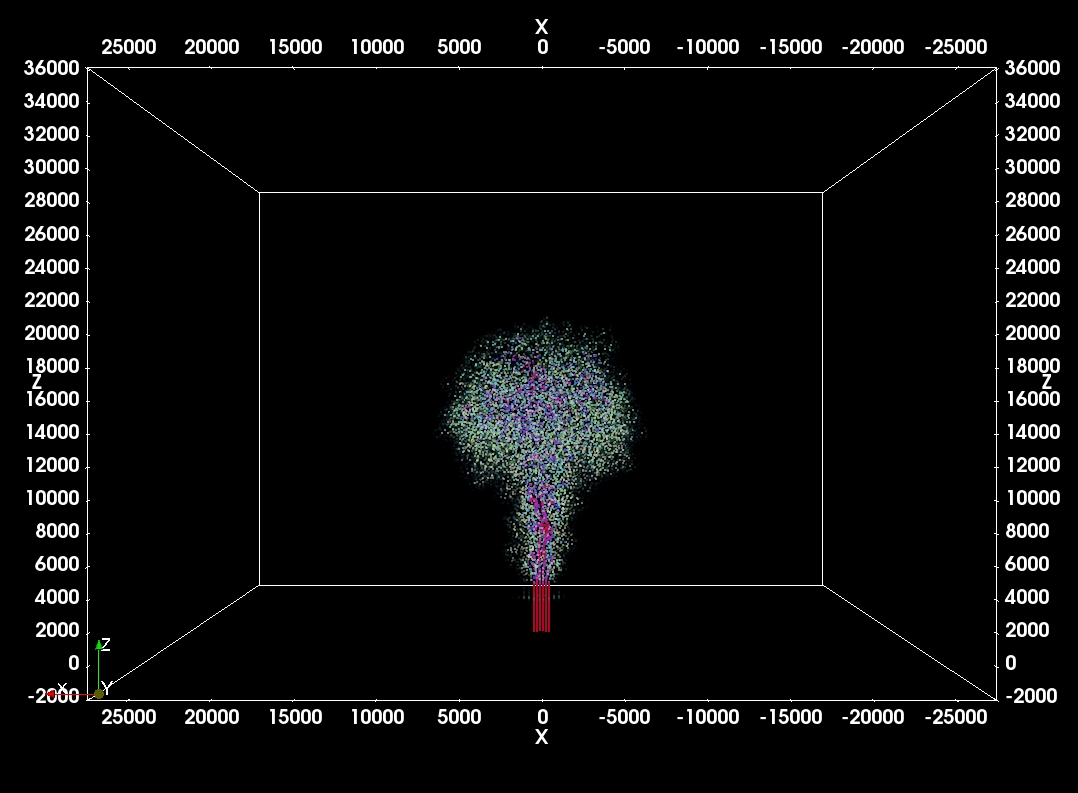
\includegraphics[width=0.99 \textwidth]{Chapter-6/Figures/ShortErupt/Erupt300_t150}
    \end{minipage}%
    \\
    \begin{minipage}{.33 \textwidth}
        \centering
        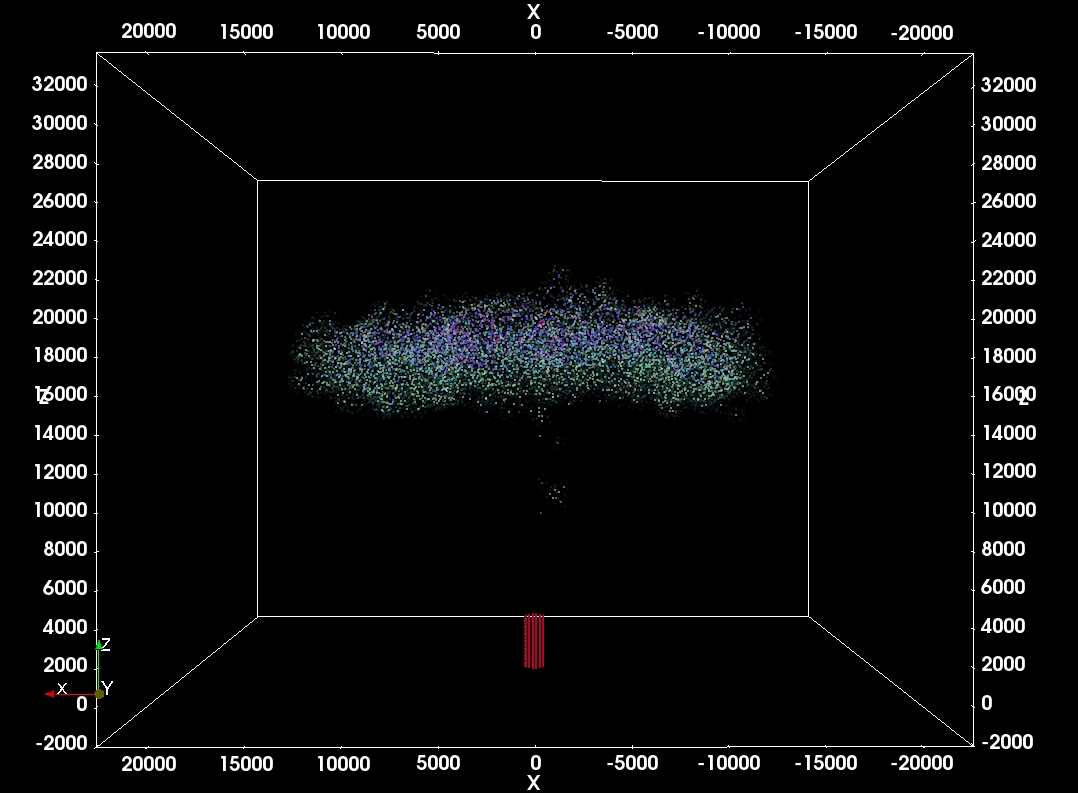
\includegraphics[width=0.99 \textwidth]{Chapter-6/Figures/ShortErupt/Erupt100_t300}
    \end{minipage}%
    \begin{minipage}{.33 \textwidth}
        \centering
        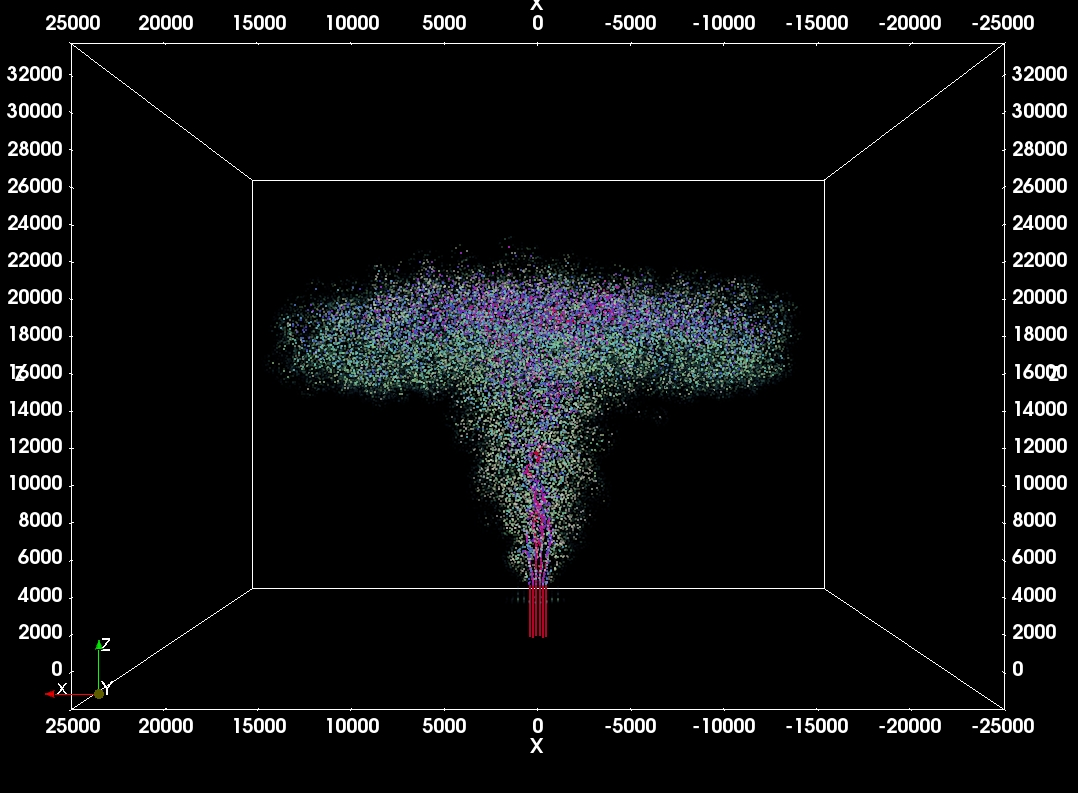
\includegraphics[width=0.99 \textwidth]{Chapter-6/Figures/ShortErupt/Erupt300_t300}
    \end{minipage}%
    \\
    \begin{minipage}{.33\textwidth}
        \centering
        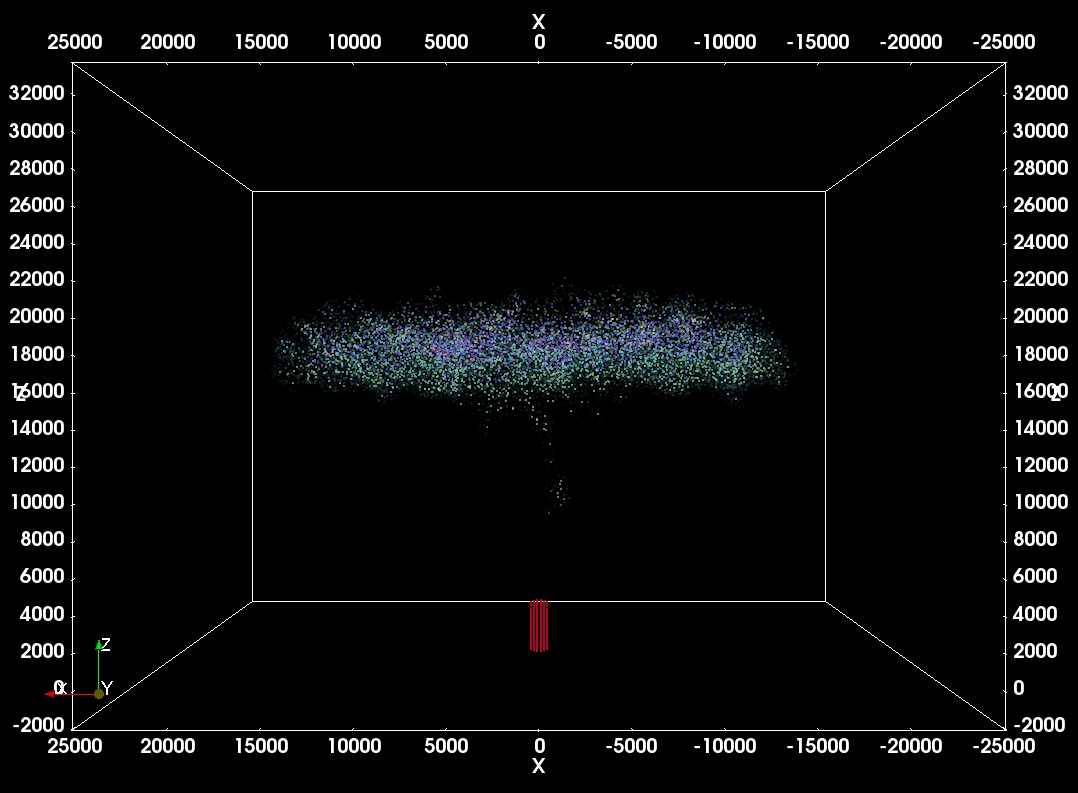
\includegraphics[width=0.99 \textwidth]{Chapter-6/Figures/ShortErupt/Erupt100_t350}
    \end{minipage}%
    \begin{minipage}{.33 \textwidth}
        \centering
        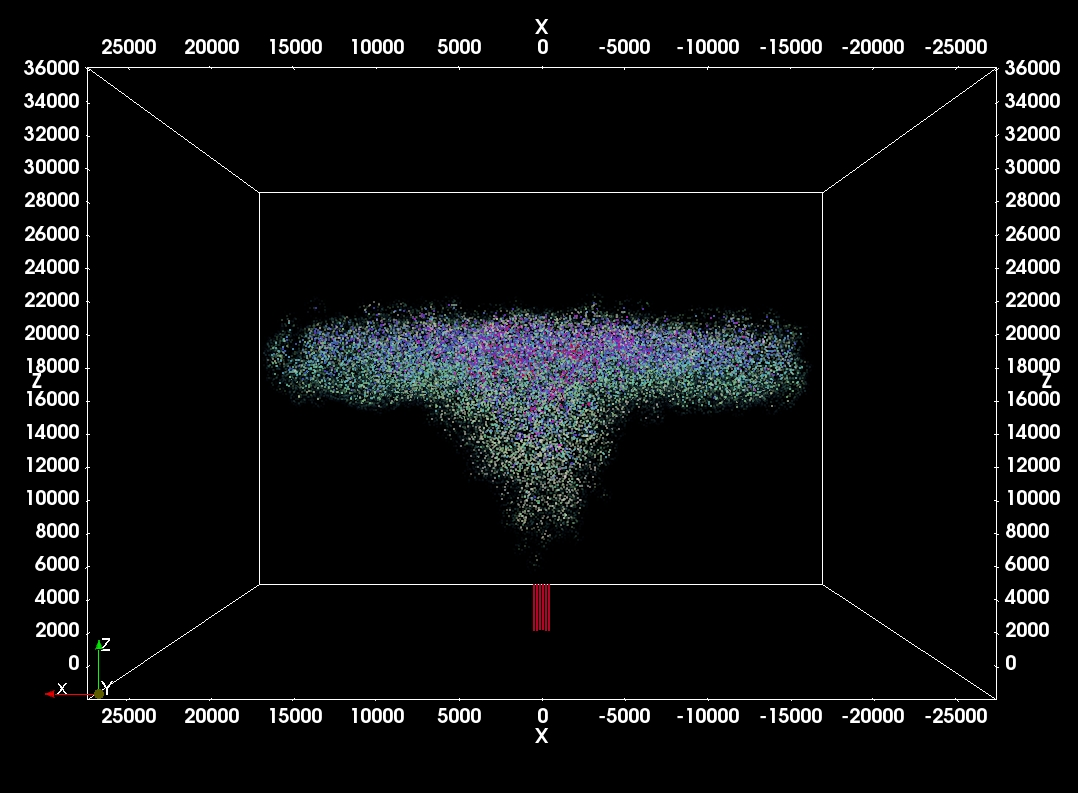
\includegraphics[width=0.99 \textwidth]{Chapter-6/Figures/ShortErupt/Erupt300_t350}
    \end{minipage}%
    \\
    \begin{minipage}{.33\textwidth}
        \centering
        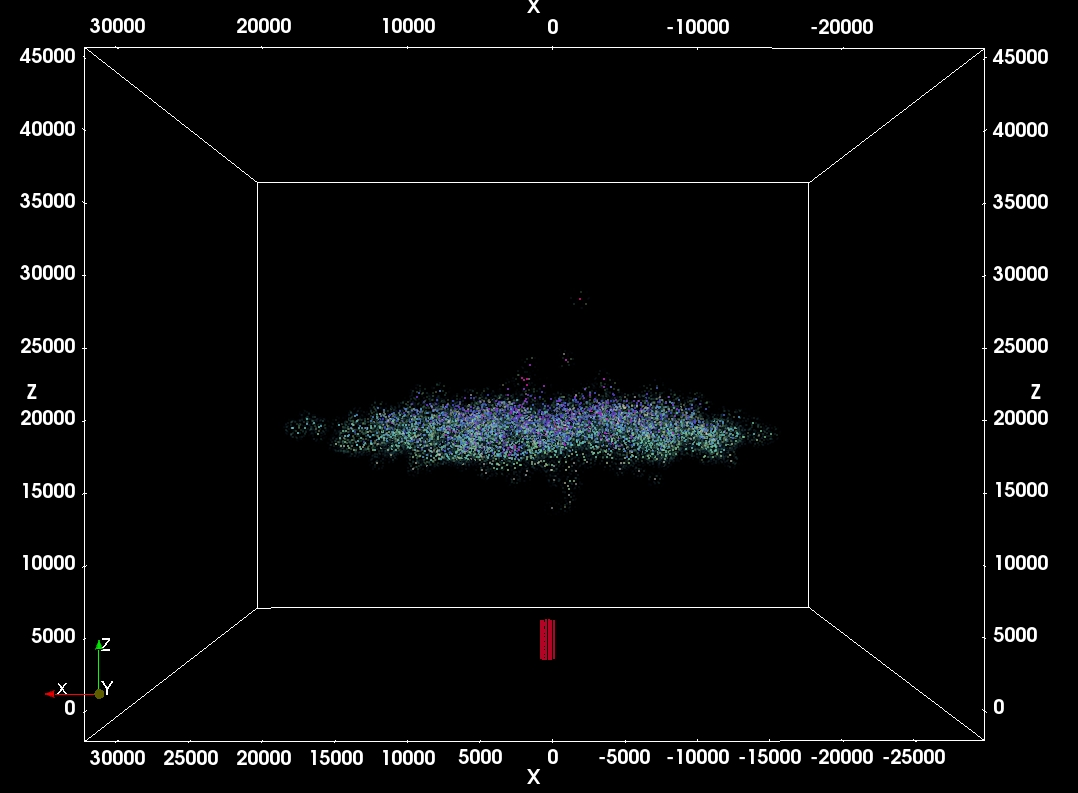
\includegraphics[width=0.99 \textwidth]{Chapter-6/Figures/ShortErupt/Erupt100_t550}
    \end{minipage}%
    \begin{minipage}{.33 \textwidth}
        \centering
        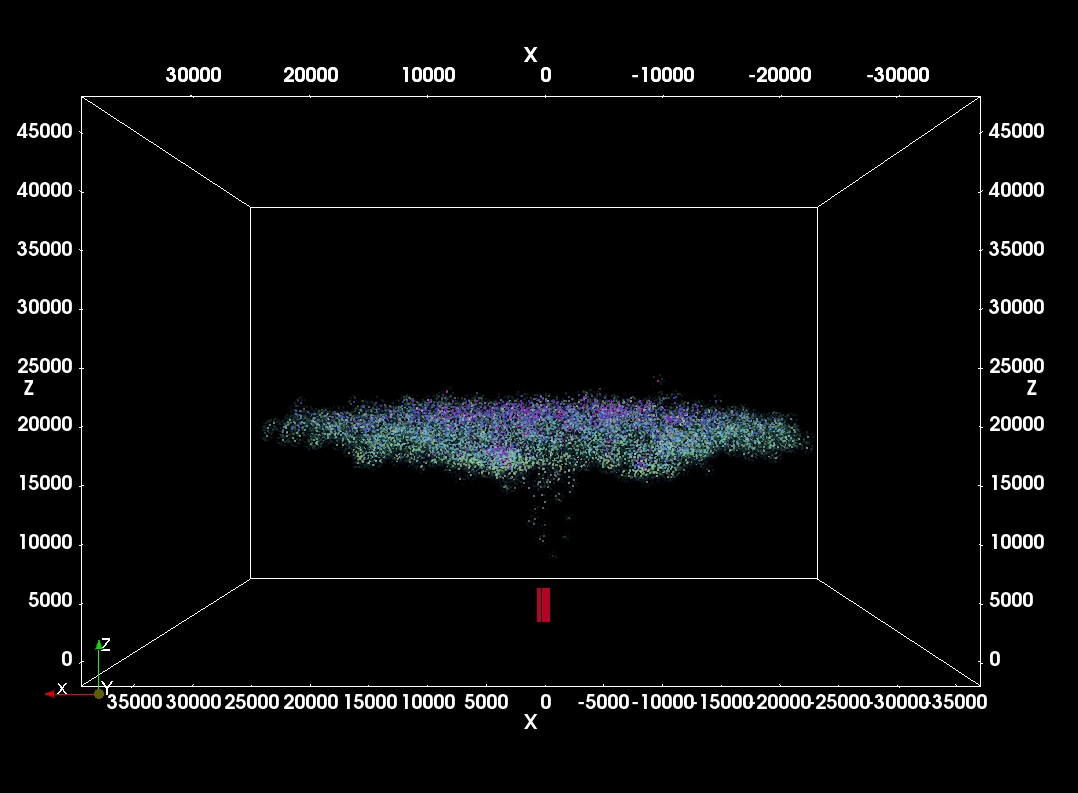
\includegraphics[width=0.99 \textwidth]{Chapter-6/Figures/ShortErupt/Erupt300_t550}
    \end{minipage}%
    \\
    \caption{Evolution of volcano plume for short periods eruption. The pictures on the left are corresponding to eruption duration of $100s$ while the right ones are for eruption duration of $300s$. Plume shape at different time is on different rows. From top to bottom, the corresponding time are $100s$ (when the left plume stops ejecting erupted material), $150s$, $300s$ (when the right plume stops ejecting erupted material), $350s$ and $550s$} 
    \label{fig:pinatubo-short-erupt-evolution}
\end{figure}

All of the previous results are simulations of successive eruptions from beginning to end. In this subsection, two short periods (100s and 300s) eruptions are simulated to further investigate the capability of Plume-SPH in capturing the salient physics in volcanic plume development. In these simulations, parameters including eruption condition, material properties, atmosphere condition, resolution and domain specifications are the same as previous simulation. The only difference is that these eruptions end during the middle of simulation. Such short period eruption cases are simulated by stopping adding new eruption ghost particles at specific time during simulation.

As has been shown in Fig. \ref{fig:pinatubo-short-erupt-evolution}, both plumes keep raising up after stopping eruption, which excludes "push" of newly erupted material from driven forces that keeps plume raising up. The NBL of two short periods eruption are the same being around $17 km \sim 24 km$, which is consistent with observations. That is to say NBL is independent of eruption duration.

\subsection{GSPH and RSPH simulation}
We also attempt to simulate the Pinatubo eruption using GSPH solver and RSPH solver. However, the simulation quickly breaks down due to negative energy. Several changes are tried to get rid of negative energy.
We notice that the negative pressure does not show up if turbulence model is removed. That is to say, the turbulent stress term $\Phi_{ab}$ and the turbulent heat exchange term $C_p \dfrac{dT}{dt}$ are removed from discretized governing equations. In addition, the velocity filtering step (Eq. \ref{eq:turbulence-v-filter}) and corresponding energy filtering step are also excluded. However, as expected, the plume collapses when turbulence model is excluded. Adding an extra energy smoothing step, which has similar effect as physical heat exchange, helps prevent plume collapse. The smoothing length for the extra averaging step is calibrated to make the plume rise  to expected height. The smoothing length is calibrated to be $\frac{1}{4}$  of the normal smoothing length.

\begin{figure}
\center
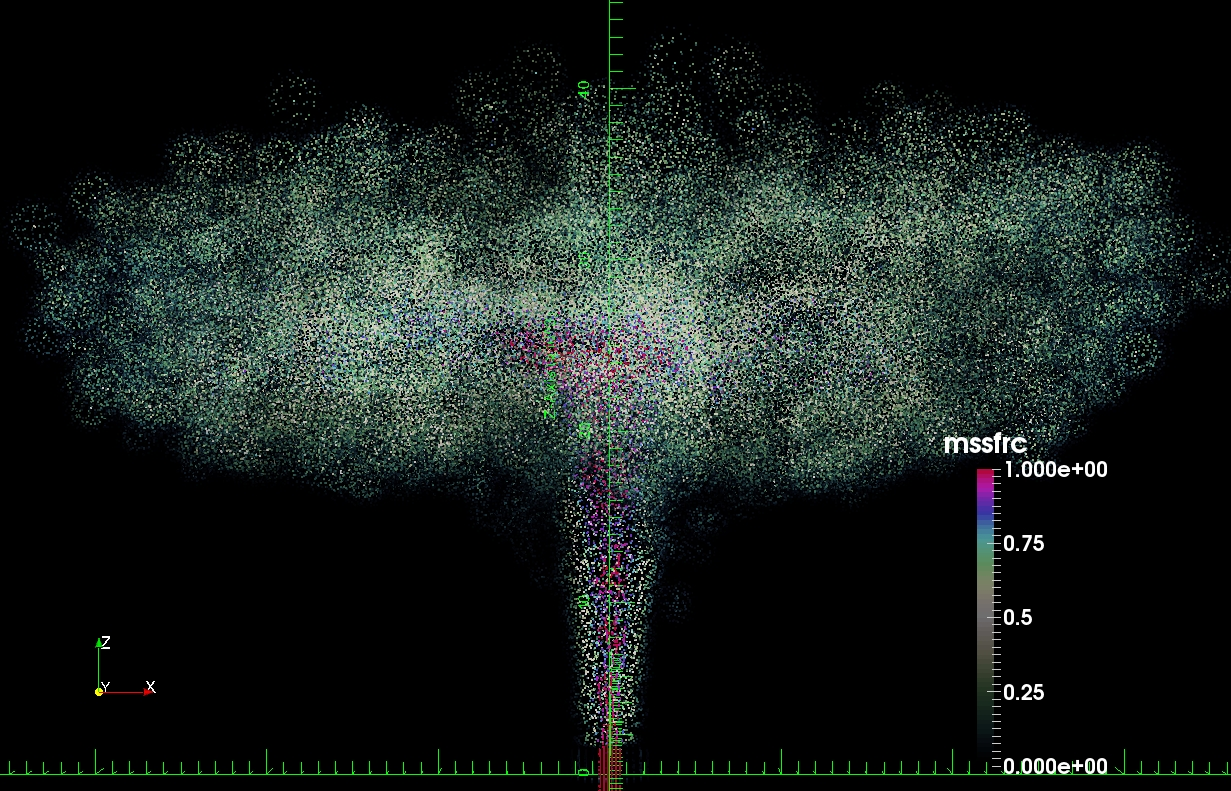
\includegraphics[width=0.75 \textwidth]{Chapter-6/Figures/RSPH_mssfrc_420s}
\caption{Plume of Pinatubo eruption simulated by RSPH method without turbulence model. An extra internal energy smoothing step is included.}
\label{fig:Pinatubo-RSPH}
\end{figure}

\begin{figure}
\center
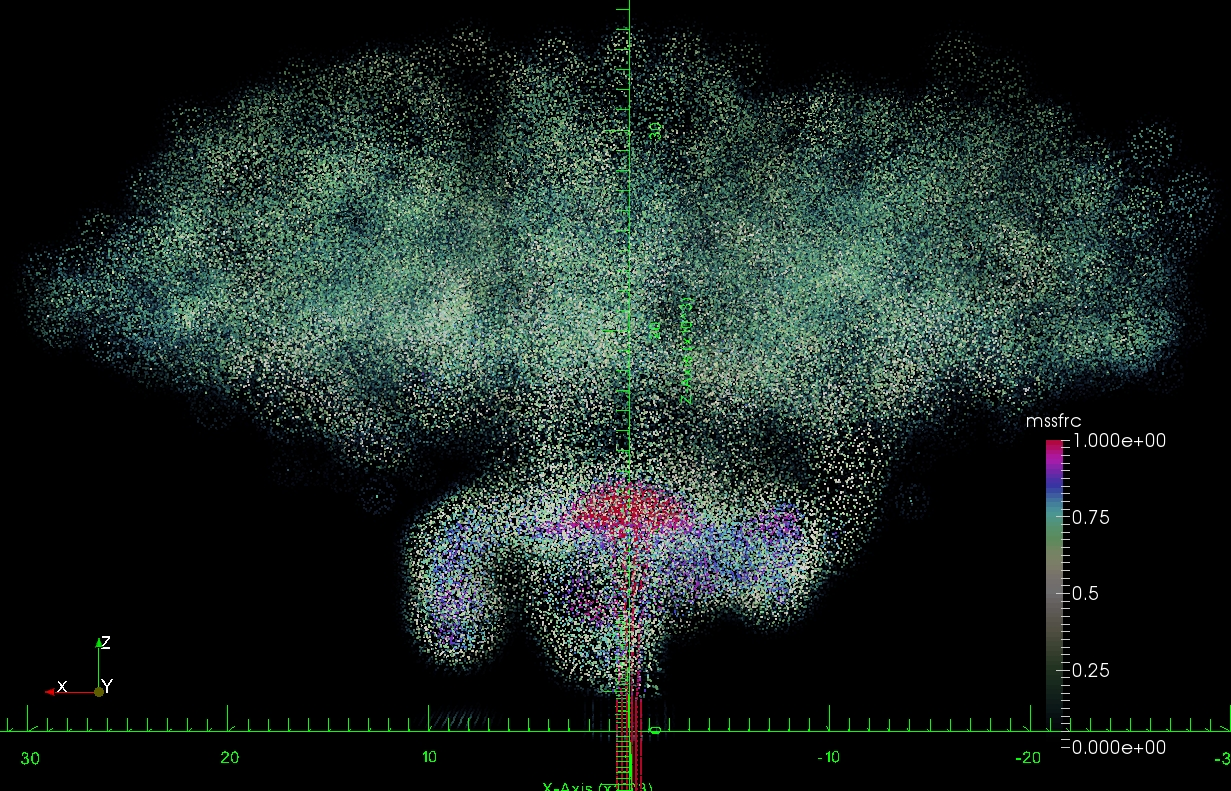
\includegraphics[width=0.75 \textwidth]{Chapter-6/Figures/GSPH_mssfrc_640s}
\caption{Plume of Pinatubo eruption simulated by GSPH method without turbulence model. An extra internal energy smoothing step is included.}
\label{fig:Pinatubo-GSPH}
\end{figure}

The volcano plume simulated by RSPH and GSPH are shown in Fig. \ref{fig:Pinatubo-RSPH} and Fig. \ref{fig:Pinatubo-GSPH}. 
All input parameters for these two simulations, including eruption condition, material properties and atmosphere data are the same as the strong-plume-no-wind case in a comparison study on eruptive column models by \citet{costa2016results}.
The maximum height and NBL of both are close to observation. However, the plume development partten simulated by GSPH is different that by SPH and RSPH. There is a more obvious stable column regime which is characterized by the suspended flow of the inner dense core. In addition, the height of the stable column simulated by GSPH is obviously lower that that predicted by RSPH and SPH. The much lower stable column height is closer to that obtained by \citet{suzuki2005numerical}.

%\section{Eyjafjallaj$\ddot{o}$kull eruption in 2010}
%Another case study is carried out in this section. Plume-SPH is used to simulate the summit explosive eruption during the second phase of Eyjafjallaj$\ddot{o}$kull eruption beginning at sometime between about midnight and sunrise on 14 April 2010. This strong or paroxysmal phase continued until 18 April. The discharge condition during this phase is variable \citep{bursik2012estimation} according to observation made over these days. Plume-SPH currently is not able to assigning eruption condition as a function of time. Single value eruption condition is adopted in the following simulation.
%Following \citet{{bursik2012estimation}}, the IMO Keflavik radiosonde from 14 April 00Z is used as atmosphere data. The radiosonde is the closest weather data both spatially and temporally to the early period of the eruption between about midnight and 07Z, and therefore best represents the nearvent weather conditions.
%The physical property of atmosphere and erupted material are the same as those adopted in Pinatubo eruption simulation (see Table \ref{tab:material_properties}). 
%As for the eruption condition, Temperature calculations \citep{keiding2012geothermobarometry} indicate the magmatic temperatures of around $1170^\circ$C (\pm $25^\circ$C) and a narrow temperature range (<$30^\circ$C) at any given depth. In contrast, benmoritic products crystallized at lower temperatures ( $1000–1060^\circ$C). Considering the cooling effect due to ice melting, we adopt the smaller value $1000^\circ$C. The eruption is actually an over pressured eruption with an average pressure higher than surrouding atmosphere. An pressure equal to that of surrounding atmosphere is adopted in simulation. Magmatic water concentrations were estimated with plagioclase-melt hygrometry by \citet{keiding2012geothermobarometry}. The maximum average water content of $1.8 \% H_2O$, obtained in one of the summit samples, is in agreement with melt inclusion observations. Such upper bound value is adopted in our simulation considering that melting ice might contribute to the water. concentration of the plume. The average value of eruption velocity and vent radius in an uncertainty qualification analysis of Eyjafjallaj$\ddot{o}$kull eruption is adopted as corresponding eruption conditions. A summary on all eruption conditions are show in Table \ref{tab:input_parameters}.
